% !TeX spellcheck = en_US
\addscenariosection{1}{Clash/Alliance Scenario}{Shattered Alliance}{\images/implosion.png}

\begin{multicols*}{2}

\textbf{Author:} Laamakala

\textit{Once united, the great kingdoms of Aldara now stand divided. Betrayal and ambition fuel the fires of war — who will forge a new order?}  % no-check-caps

\subsection*{\MakeUppercase{Scenario Length}}
This Scenario plays out over 14 Rounds.

\subsection*{\MakeUppercase{Player Setup}}
\textbf{Player Count:} 6P FFA, 2v2v2 Alliance.

\textbf{Starting Resources:} 10 \svg{gold}, 2 \svg{building_materials}, 1 \svg{valuables}

\textbf{Starting Income:} 10 \svg{gold}, 0 \svg{building_materials}, 0 \svg{valuables}

\textbf{Starting Units:}

\begin{itemize}
  \item 2 × Chosen Neutral \bronze Unit from the closest starting player's Faction
\end{itemize}

\textbf{Town Buildings:} Citadel

\textbf{Map Tile Pool:} Each player takes 3 random Far (II-III) Map Tiles.

\subsection*{\MakeUppercase{Map Setup}}
Take the following Map Tiles and arrange them as shown in the Scenario map layout:

\begin{itemize}
  \item 6 × Starting (I) Map Tiles
  \item 12 × Near (IV-V) Map Tiles
  \item 3 × Center (VI-VII) Map Tiles
\end{itemize}

\subsection*{\MakeUppercase{Victory Conditions}}
The game ends when any of the following conditions are met:
\begin{itemize}
  \item One player has defeated each other player's Main Hero once. \textit{That player wins the game immediately.}
  \item At the end of Round 14.
\end{itemize}

\subsection*{\MakeUppercase{Victory Points}}
If no player has achieved immediate victory, the player with the most Victory Points (VPs) wins. When the game ends, the players gain:
\begin{itemize}
  \item 3 VP for winning a Level VII Combat.
  \item 2 VP for defeating the Main Hero of your closest starting player. \textit{Once per Faction.}
  \item 1 VP for defeating another player's Main Hero. \textit{One per enemy.}
  \item 1 VP for possession of the Grail Token.
\end{itemize}

\subsection*{\MakeUppercase{Timed Events}}
\textbf{End of \nth{2} Round:}
\begin{itemize}
  \item Each player may resolve all Fields their closest starting player visited this Round. (Do not increase any income.)
\end{itemize}
\textbf{\nth{5} Round:}
\begin{itemize}
  \item Remove all Black Cubes from the map except those on Learning Stones.
\end{itemize}
\textbf{End of \nth{6} Round:}
\begin{itemize}
  \item Each player may resolve one Field their closest starting player visited this Round. (Do not increase any income.)
\end{itemize}
\textbf{\nth{7} Round:}
\begin{itemize}
  \item Each player may recruit one Neutral \silver\ Unit from their closest starting player's Faction for half its recruitment cost.
\end{itemize}
\textbf{\nth{11} Round:}
\begin{itemize}
  \item Repeat the events of Rounds 6 and 7.
\end{itemize}

\subsection*{\MakeUppercase{Additional Rules}}
\begin{itemize}
  \item Once per Round at the beginning of a Level I-III Combat, the closest starting player may change one Neutral Unit to one Neutral Unit of the same or lower Tier from their Faction.
  \item \textbf{Sanctuary:} Choose 1 \svg{spellpower} from your M\&M Deck and add it to your hand, then reshuffle your Deck. \textit{Visitable once per Faction.}
  \item \textbf{Obelisk:} Choose 1 \svg{artifact} from your M\&M Deck and add it to your hand, then reshuffle your Deck.
  \item \textbf{Dragon Utopia:} Defended only by Dragons. Recruit one Neutral Dragon you defeated for half its recruitment cost (rounded up). \textit{Trading Post conversion may be used for this}.
  \item \textbf{Random Town:} On the next Resource Round, you may recruit one \textbf{Faction Unit} from the defending Faction for free.
  \item \textbf{Level VII Settlement:} You may Reinforce one Unit for half its Recruitment cost \textbf{and} increase all incomes by one space.
  \item Level VII Neutral Combats cannot be skipped.
\end{itemize}

\begin{center}
  \vspace*{\fill}
  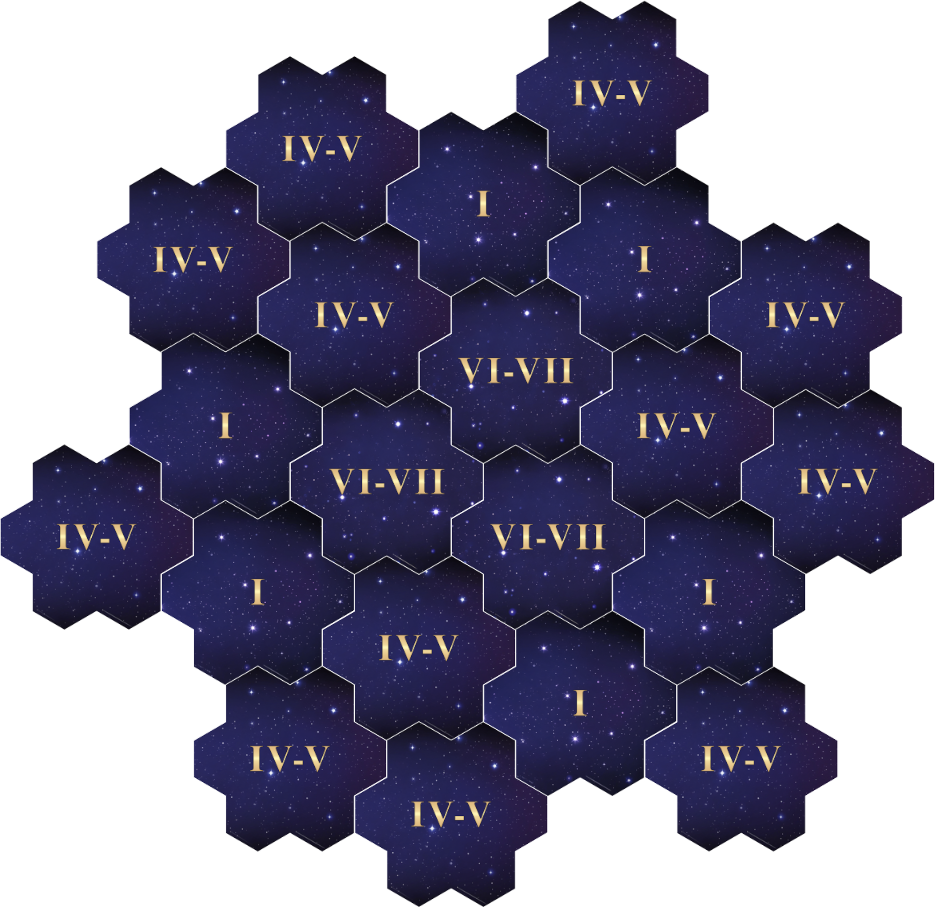
\includegraphics[width=1.0\linewidth]{\maps/shattered_alliance-6p.png}
  \captionof{figure}{\textbf{SCENARIO MAP LAYOUT}}
  \vspace*{\fill}
\end{center}

\columnbreak

\begin{itemize}
  \item \textbf{Grail Token:} When gained, draw Cards up to your \svg{hand} limit. If you start your turn with the Grail Token, gain \svg{morale_positive}, 10 \svg{gold}, and 2 \svg{valuables}. If a Hero carrying the Grail Token is defeated, the Grail Token is given to the winner of that Combat.
  \item If a Hero with the Grail Token uses Dimension Door, Fly, or Town Portal, the Grail Token is dropped on the origin Field before the Hero moves.
  \item A defeated Main Hero may Empower one Statistic Card from their Deck of M\&M.
  \item With fewer than 6 players, the unused Starting Towns are defended exactly as a Random Town.
  \item Flagging an unused Starting Town increases two separate incomes by 1 space.
  \item When a Hero moves to a Starting Town, that Hero gains +1 \svg{movement}.
  \item \textit{"Closest starting player" is the player whose starting Tile is closest to your starting Tile.}
\end{itemize}

\vspace*{\fill}

\begin{center}
  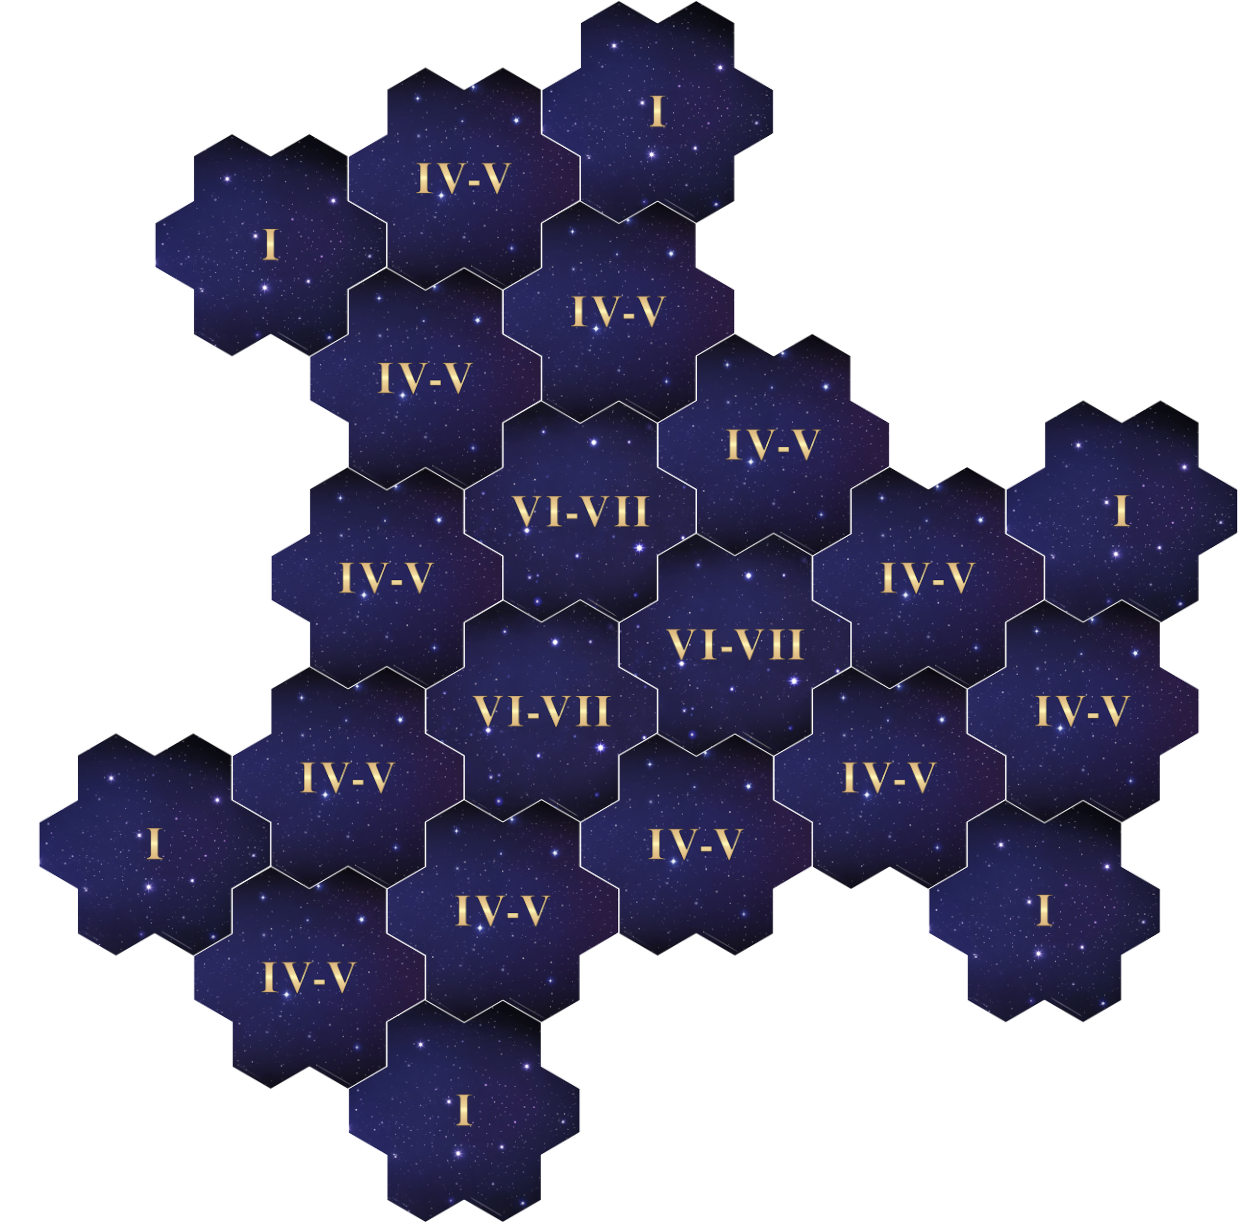
\includegraphics[width=1.05\linewidth]{\maps/shattered_alliance_alt-6p.png}
  \captionof{figure}{\textbf{ALTERNATIVE MAP LAYOUT}}
  \vspace*{\fill}
\end{center}

\end{multicols*}
